\begin{figure}[H]
\centering
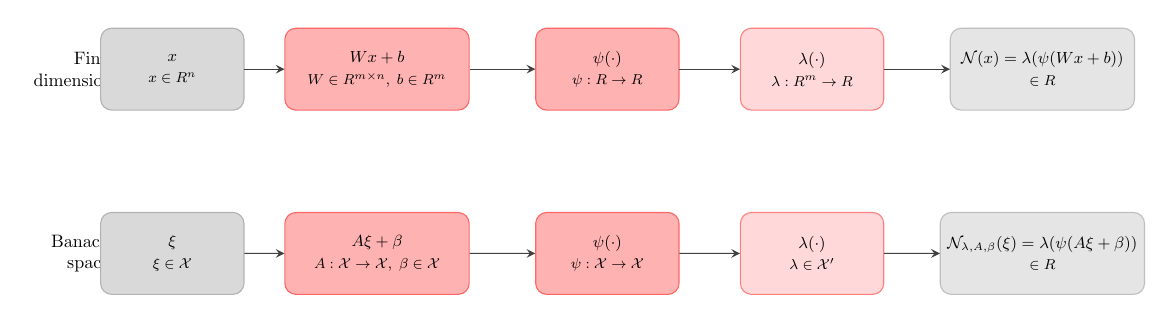
\begin{tikzpicture}[
    scale=0.65,
    transform shape,
    box/.style={rectangle, rounded corners=4pt, minimum width=28mm, minimum height=16mm, inner sep=4pt, align=center},
    >=stealth
]
\definecolor{darkgrey}{RGB}{90,90,90}

% ======================
% TOP ROW: Finite-dimensional
% ======================
\node[font=\normalsize, align=right] at (-1.8, 0.0)
    {Finite-\\dimensional};

% Input
\node[box, fill=gray!30, draw=gray!60] (FI) at (0, 0)
    {\small$x$\\\footnotesize$x \in \mathbb{R}^n$};

% Affine step
\node[box, fill=red!30, draw=red!60, minimum width=36mm] (FA) at (4, 0)
    {\small$Wx + b$\\\footnotesize$W \in \mathbb{R}^{m \times n},\; b \in \mathbb{R}^m$};

% Activation
\node[box, fill=red!30, draw=red!60] (FP) at (8.5, 0)
    {\small$\psi(\cdot)$\\\footnotesize$\psi : \mathbb{R} \to \mathbb{R}$};

% Linear functional
\node[box, fill=red!15, draw=red!50] (FL) at (12.5, 0)
    {\small$\lambda(\cdot)$\\\footnotesize$\lambda : \mathbb{R}^m \to \mathbb{R}$};

% Output
\node[box, fill=gray!20, draw=gray!50, minimum width=36mm] (FO) at (17.0, 0)
    {\small$\mathcal{N}(x) = \lambda(\psi(Wx+b))$\\\footnotesize$\in \mathbb{R}$};

% Arrows top row
\draw[->, draw=darkgray] (FI) -- (FA);
\draw[->, draw=darkgray] (FA) -- (FP);
\draw[->, draw=darkgray] (FP) -- (FL);
\draw[->, draw=darkgray] (FL) -- (FO);

% ======================
% BOTTOM ROW: Banach space
% ======================
\node[font=\normalsize, align=right] at (-1.8, -3.6)
    {Banach\\space};

% Input
\node[box, fill=gray!30, draw=gray!60] (BI) at (0, -3.6)
    {\small$\xi$\\\footnotesize$\xi \in \mathcal{X}$};

% Affine step
\node[box, fill=red!30, draw=red!60, minimum width=36mm] (BA) at (4, -3.6)
    {\small$A\xi + \beta$\\\footnotesize$A : \mathcal{X} \to \mathcal{X},\; \beta \in \mathcal{X}$};

% Activation
\node[box, fill=red!30, draw=red!60] (BP) at (8.5, -3.6)
    {\small$\psi(\cdot)$\\\footnotesize$\psi : \mathcal{X} \to \mathcal{X}$};

% Linear functional
\node[box, fill=red!15, draw=red!50] (BL) at (12.5, -3.6)
    {\small$\lambda(\cdot)$\\\footnotesize$\lambda \in \mathcal{X}'$};

% Output
\node[box, fill=gray!20, draw=gray!50, minimum width=36mm] (BO) at (17.0, -3.6)
    {\small$\mathcal{N}_{\lambda,A,\beta}(\xi) = \lambda(\psi(A\xi+\beta))$\\\footnotesize$\in \mathbb{R}$};

% Arrows bottom row
\draw[->, draw=darkgray] (BI) -- (BA);
\draw[->, draw=darkgray] (BA) -- (BP);
\draw[->, draw=darkgray] (BP) -- (BL);
\draw[->, draw=darkgray] (BL) -- (BO);

\end{tikzpicture}
\caption{Correspondence between the finite-dimensional neuron
$\mathcal{N}(x) = \lambda(\psi(Wx+b))$ and its infinite-dimensional
analogue $\mathcal{N}_{\lambda,A,\beta}(\xi) = \lambda(\psi(A\xi+\beta))$
on a Banach space $\mathcal{X}$. Each ingredient in the finite-dimensional
setting has a direct Banach-space counterpart: the matrix $W$ becomes a
bounded linear operator $A:\mathcal{X}\to\mathcal{X}$, the bias $b$
becomes an element $\beta\in\mathcal{X}$, and the linear functional
$\lambda:\mathbb{R}^m\to\mathbb{R}$ becomes a continuous linear
functional $\lambda\in\mathcal{X}'$.}
\label{fig:neuron_analogy}
\end{figure}